%%%%%%%%%%%%%%%%%%%%%%%%%%%%%%%%%%%%%%%%%
% Programming/Coding Assignment
% LaTeX Template
%
% This template has been downloaded from:
% http://www.latextemplates.com
%
% Original author:
% Ted Pavlic (http://www.tedpavlic.com)
%
% Note:
% The \lipsum[#] commands throughout this template generate dummy text
% to fill the template out. These commands should all be removed when
% writing assignment content.
%
% This template uses a Perl script as an example snippet of code, most other
% languages are also usable. Configure them in the "CODE INCLUSION
% CONFIGURATION" section.
%
%%%%%%%%%%%%%%%%%%%%%%%%%%%%%%%%%%%%%%%%%

%----------------------------------------------------------------------------------------
%	PACKAGES AND OTHER DOCUMENT CONFIGURATIONS
%----------------------------------------------------------------------------------------

\documentclass{article}

\usepackage{fancyhdr} % Required for custom headers
\usepackage{lastpage} % Required to determine the last page for the footer
\usepackage{extramarks} % Required for headers and footers
\usepackage[usenames,dvipsnames]{color} % Required for custom colors
\usepackage{graphicx} % Required to insert images
\usepackage{listings} % Required for insertion of code
\usepackage{courier} % Required for the courier font
\usepackage{lipsum} % Used for inserting dummy 'Lorem ipsum' text into the template
\usepackage[utf8]{inputenc}
\usepackage{amsmath,amssymb,amsfonts,amsthm,graphicx,enumitem}
\usepackage[parfill]{parskip}
\usepackage{color}
\usepackage{float}
\usepackage[ruled,vlined]{algorithm2e}
% Margins
\topmargin=-0.45in
\evensidemargin=0in
\oddsidemargin=0in
\textwidth=6.5in
\textheight=9.0in
\headsep=0.25in

\linespread{1.1} % Line spacing

% Set up the header and footer
\pagestyle{fancy}
\lhead{\hmwkAuthorName} % Top left header
\chead{\hmwkClass\ (\hmwkClassInstructor\ \hmwkClassTime): \hmwkTitle} % Top center head
\rhead{\firstxmark} % Top right header
\lfoot{\lastxmark} % Bottom left footer
\cfoot{} % Bottom center footer
\rfoot{Page\ \thepage\ of\ \protect\pageref{LastPage}} % Bottom right footer
\renewcommand\headrulewidth{0.4pt} % Size of the header rule
\renewcommand\footrulewidth{0.4pt} % Size of the footer rule

\setlength\parindent{0pt} % Removes all indentation from paragraphs

%----------------------------------------------------------------------------------------
%	CODE INCLUSION CONFIGURATION
%----------------------------------------------------------------------------------------

\definecolor{MyDarkGreen}{rgb}{0.0,0.4,0.0} % This is the color used for comments
\lstloadlanguages{Perl} % Load Perl syntax for listings, for a list of other languages supported see: ftp://ftp.tex.ac.uk/tex-archive/macros/latex/contrib/listings/listings.pdf
\lstset{language=Perl, % Use Perl in this example
        frame=single, % Single frame around code
        basicstyle=\small\ttfamily, % Use small true type font
        keywordstyle=[1]\color{Blue}\bf, % Perl functions bold and blue
        keywordstyle=[2]\color{Purple}, % Perl function arguments purple
        keywordstyle=[3]\color{Blue}\underbar, % Custom functions underlined and blue
        identifierstyle=, % Nothing special about identifiers
        commentstyle=\usefont{T1}{pcr}{m}{sl}\color{MyDarkGreen}\small, % Comments small dark green courier font
        stringstyle=\color{Purple}, % Strings are purple
        showstringspaces=false, % Don't put marks in string spaces
        tabsize=5, % 5 spaces per tab
        %
        % Put standard Perl functions not included in the default language here
        morekeywords={rand},
        %
        % Put Perl function parameters here
        morekeywords=[2]{on, off, interp},
        %
        % Put user defined functions here
        morekeywords=[3]{test},
       	%
        morecomment=[l][\color{Blue}]{...}, % Line continuation (...) like blue comment
        numbers=left, % Line numbers on left
        firstnumber=1, % Line numbers start with line 1
        numberstyle=\tiny\color{Blue}, % Line numbers are blue and small
        stepnumber=5 % Line numbers go in steps of 5
}

% Creates a new command to include a perl script, the first parameter is the filename of the script (without .pl), the second parameter is the caption
\newcommand{\perlscript}[2]{
\begin{itemize}
\item[]\lstinputlisting[caption=#2,label=#1]{#1.pl}
\end{itemize}
}

%----------------------------------------------------------------------------------------
%	DOCUMENT STRUCTURE COMMANDS
%	Skip this unless you know what you're doing
%----------------------------------------------------------------------------------------

% Header and footer for when a page split occurs within a problem environment
\newcommand{\enterProblemHeader}[1]{
\nobreak\extramarks{#1}{#1 continued on next page\ldots}\nobreak
\nobreak\extramarks{#1 (continued)}{#1 continued on next page\ldots}\nobreak
}

% Header and footer for when a page split occurs between problem environments
\newcommand{\exitProblemHeader}[1]{
\nobreak\extramarks{#1 (continued)}{#1 continued on next page\ldots}\nobreak
\nobreak\extramarks{#1}{}\nobreak
}

\setcounter{secnumdepth}{0} % Removes default section numbers
\newcounter{homeworkProblemCounter} % Creates a counter to keep track of the number of problems

\newcommand{\homeworkProblemName}{}
\newenvironment{homeworkProblem}[1][Problem \arabic{homeworkProblemCounter}]{ % Makes a new environment called homeworkProblem which takes 1 argument (custom name) but the default is "Problem #"
\stepcounter{homeworkProblemCounter} % Increase counter for number of problems
\renewcommand{\homeworkProblemName}{#1} % Assign \homeworkProblemName the name of the problem
\section{\homeworkProblemName} % Make a section in the document with the custom problem count
\enterProblemHeader{\homeworkProblemName} % Header and footer within the environment
}{
\exitProblemHeader{\homeworkProblemName} % Header and footer after the environment
}

\newcommand{\problemAnswer}[1]{ % Defines the problem answer command with the content as the only argument
\noindent\framebox[\columnwidth][c]{\begin{minipage}{0.98\columnwidth}#1\end{minipage}} % Makes the box around the problem answer and puts the content inside
}

\newcommand{\homeworkSectionName}{}
\newenvironment{homeworkSection}[1]{ % New environment for sections within homework problems, takes 1 argument - the name of the section
\renewcommand{\homeworkSectionName}{#1} % Assign \homeworkSectionName to the name of the section from the environment argument
\subsection{\homeworkSectionName} % Make a subsection with the custom name of the subsection
\enterProblemHeader{\homeworkProblemName\ [\homeworkSectionName]} % Header and footer within the environment
}{
\enterProblemHeader{\homeworkProblemName} % Header and footer after the environment
}

%----------------------------------------------------------------------------------------
%	NAME AND CLASS SECTION
%----------------------------------------------------------------------------------------

\newcommand{\hmwkTitle}{Assignment\ \#2} % Assignment title
\newcommand{\hmwkDueDate}{Today} % Due date
\newcommand{\hmwkClass}{NPDE for Option Pricing } % Course/class
\newcommand{\hmwkClassTime}{12:20am} % Class/lecture time
\newcommand{\hmwkClassInstructor}{Instructor:Dr.Kopriva} % Teacher/lecturer
\newcommand{\hmwkAuthorName}{Jian Wang } % Your name

%----------------------------------------------------------------------------------------
%	TITLE PAGE
%----------------------------------------------------------------------------------------

\title{
\vspace{2in}
\textmd{\textbf{\hmwkClass:\ \hmwkTitle}}\\
\normalsize\vspace{0.1in}\small{Due\ on\ \hmwkDueDate}\\
\vspace{0.1in}\large{\textit{\hmwkClassInstructor\ \hmwkClassTime}}
\vspace{3in}
}

\author{\textbf{\hmwkAuthorName}}
\date{} % Insert date here if you want it to appear below your name

%----------------------------------------------------------------------------------------

\begin{document}

\maketitle

%----------------------------------------------------------------------------------------
%	TABLE OF CONTENTS
%----------------------------------------------------------------------------------------

%\setcounter{tocdepth}{1} % Uncomment this line if you don't want subsections listed in the ToC

\newpage
\tableofcontents
\newpage

%% insert the programming code
%\begin{homeworkProblem}
%Listing \ref{homework_example} shows a Perl script.
%
%\perlscript{homework_example}{Sample Perl Script With Highlighting}
%
%\lipsum[1]
%\end{homeworkProblem}

%% insert the chart
%\begin{homeworkProblem}
%\lipsum[2]
%
%\problemAnswer{
%\begin{center}
%\includegraphics[width=0.75\columnwidth]{example_figure} % Example image
%\end{center}
%\lipsum[3-5]
%}
%\end{homeworkProblem}
%% Example of list array and emurate
%\begin{homeworkProblem}
%
%\begin{flalign}
%A =
%\begin{bmatrix}
%A_{11} & A_{21} \\
%A_{21} & A_{22}
%\end{bmatrix}
%\end{flalign}
%
%\begin{itemize}
%	\item First item in a list
%		\begin{itemize}
%		\item First item in a list
%			\begin{itemize}
%			\item First item in a list
%			\item Second item in a list
%			\end{itemize}
%		\item Second item in a list
%		\end{itemize}
%	\item Second item in a list
%\end{itemize}
%
%\begin{enumerate}
%\item First item in a list
%\item Second item in a list
%\item Third item in a list
%\end{enumerate}

%% equation formula
%$\left \{
%\begin{tabular}{l}
%$V_t+\frac{\sigma^2S^2}{2}V_{SS}+rSV_s - rV=0$\\
%
%$V(0,t)=e^{-r(T-t)}$\\
%
%$V(\infty,t)=0$\\
%
%$V(S,T)=I_{\{S\leq K\}}$
%\end{tabular}
%\right.$

%\end{homeworkProblem}
%----------------------------------------------------------------------------------------

\begin{homeworkProblem}

\section*{[Summary]}
1) The iterative number of PSOR algorithm was first decreasing and then increasing according to the increasing of the overrelaxation  parameters.\\

2)We may need 4096 points and 160 time steps to ensure the 4 digit numbers of both American and European option.\\

3) The value of American put option was higher than the value of the European put option.\\

4) When stock price was less than the optimal exercise boundary, the American option price was same as the payoff function, the delta was -1 and gamma remain 0. Gamma will increase dramatically when $S>S_f$

\section*{[Statement of the problem]}
1. Repeat the computation of the price of the European vanilla put in the last assignment and compare the CPU time for computing the American VS the European option. For the PSOR, test the sensitivity of the CPU time based on the optimal relaxation parameter and the iteration tolerance.\\

2.Compute and plot the values of the European and American vanilla put for K =\$10, r= 0.1/yr, $\sigma$ =0.4/$\sqrt{yr}$ amd wotj a six month expiry with ranacher smoothing for S $\in$ [0,2K]. Compute the greeks, $\Delta$ and $\Gamma$ for both. Compare and discuss the solutions. Test the sufficient number of points and time steps so that the European option has four significant digits. Test if the American option also converged with this grid. If not, how many points and time steps are required?\\

3. Calculate the optimal exercise boundary as a function of time. Draw the picture.\\


\section*{[Description of The Mathematics]}
The BSM and boundary condition for American put option is:\\
\begin{flalign*}
\left \{
\begin{tabular}{l}
$V_t+\frac{\sigma^2S^2}{2}V_{SS}+rSV_s - rV=0$\\
$V(0,t)=Ke^{-r(T-t)}$\\
$V(\infty,t)=0$\\
$V(S,T)=max(K-S,0)$\\
$V(s,t)=Max(V(s,t), K-s)$ for s$<$$S_{max}$ and t $<$ T\\
\end{tabular}
\right.
\end{flalign*}
\\

combine : $\delta_t^+V_j^n +L_h[\alpha V_j^{n+1}+(1-\alpha)V_j^n]=0$\\

          $\alpha =1$ : Back Euler\\
          $\alpha=\frac{1}{2}$ : Crank-Nicolson method
\\

\textbf{Backward Euler method:}\\
The scheme for the Backward Euler method is given by:\\
\begin{flalign*}
\frac{V_{i,j}-V_{i,j-1}}{\delta t}+\frac{1}{2}\sigma^2(i\delta S)^2\frac{V_{i+1,j-1}-2V_{i,j-1}+V_{i-1,j-1}}{\delta S^2}+r(i\delta S)\frac{V_{i+1,j-1}-V_{i-1}{j-1}}{2\delta S)}-rV_{i,j-1}=0\\
\end{flalign*}
we can rewrite it as:\\
\begin{flalign*}
V_{i,j}=A_{i}V_{i-1,j-1}+B_iV_{i,j-1}+C_iV_{i+1,j-1}
\end{flalign*}
where:\\

\begin{flalign*}
A_i=\frac{1}{2}\delta t (r_i-\sigma^2i^2), B_i=1+(\sigma^2i^2+r)\delta t, C_i=-\frac{1}{2}\delta t(ri+\sigma^2i^2)\\
\end{flalign*}

\textbf{Crank-Nicolson method:}\\

\begin{flalign*}
&\frac{V_{ij}-V_{i,j-1}}{\delta t}+\frac{ri\delta S}{2}+(\frac{V_{i+1,j-1}-V_{i-1,j-1}}{2\delta S}+\frac{ri\delta S}{2}(\frac{V
_{i+1,j}-V_{i-1,j}}{2\delta S})+\\
&\frac{\sigma^2 i^2 (\delta S)^2}{4}(\frac{V_{i+1,j-1}-2V_{i,j-1}+V_{i-1,j-1}}{(\delta S)^2})+\\
&\frac{\sigma^2 i^2 (\delta S)^2}{4}(\frac{V_{i+1,j}-2V_{i,j}+V_{i-1,j}}{(\delta S)^2})=\frac{r}{2}V_{i,j-1}+\frac{r}{2}V_{ij}&&
\end{flalign*}

We can  rewrite the above equation as:\\
\begin{flalign*}
-\alpha_i V_{i-1,j-1}+(1-\beta_i)V_{i,j-1}-\gamma_{i}V_{i+1,j-1}=\alpha_i V_{i-1,j}+(1+\beta_i)V_{i,j}+\gamma_{i}V_{i+1,j}
\end{flalign*}

Where: \\

\begin{flalign*}
\quad\quad &\alpha_i=\frac{\Delta t}{4}(\sigma^2i^2-ri)\\
&\beta_i=-\frac{\Delta t}{2}(\sigma^2i^2+r)\\
&\gamma_i=\frac{\Delta t}{4}(\sigma^2i^2+ri)
\end{flalign*}

\textbf{Ranacher Smooth method}\\

(1)We use backward Euler for a few n $\ge$ 2 time steps\\
(2)Use Crank-Nicolson after that: given second order accuracy \\


\textbf{Close form Black Scholes formula}

To test the result for the SDE model of the option pricing, we also need to know the close form solution of the Black -Scholes assumptions, which is the famous Black- Scholes formula. \\
For the European put options:\\
\begin{flalign*}
P(S,t)=Ke^{-r(T-t)}N(-d_2)-SN(-d_1)
\end{flalign*}\\
where:\\
\begin{flalign*}
d_1=\frac{log\frac{S}{K}+(r+\frac{1}{2}\sigma^2)(T-t)}{\sigma\sqrt{T-t}}\\
d_2=\frac{log\frac{S}{K}+(r-\frac{1}{2}\sigma^2)(T-t)}{\sigma\sqrt{T-t}}\\
N(x)=\frac{1}{\sqrt{2\pi}}\int_{-\infty}{x}e^{-\frac{1}{2}S^2}ds
\end{flalign*}
\textbf{Delta for Vanilla put option:}
\begin{flalign*}
-e^{-q \tau} \Phi(-d_1)
\end{flalign*}
\textbf{Gamma for Vanilla put option:}\\
\begin{flalign*}
-e^{-q \tau} \frac{\Phi(d_1)}{S\sigma \sqrt{\tau}}
\end{flalign*}
\textbf{Vega for Vanilla put option:}\\
\begin{flalign*}
Se^{-q \tau}\phi(d_1)\sqrt{\tau}=Ke^{-r\tau}\phi(d_2)\sqrt{\tau}
\end{flalign*}
where $q$ here is the dividend rate which is equal to 0 in our problem.\\

\section*{[Description of Algorithm]}
\clearpage
\begin{algorithm}
\DontPrintSemicolon
\Begin{
$x \longleftarrow x_0$\\
\For{k = 1 to maxiter}{
$rmax \longleftarrow 0$\\
\For {j = 1 to N-1}
{ $r= y_j- (l_j x_{j-1}+d_jx_j+u_jx_{j+1})$\\
  $x_{test}=x_j+\omega r /d_j$\\
  \If{$x_{test}>payoff_j$}{
      $x_j=x_{test}$\\
      $rmax=max(rmax,|r|)$}
  \Else
 {$x_j=payoff_j$}

 \If{$r_{max}<Tol$}
 {exit}
 }
}
}
\caption{PSOR Algoithm\label{IR}}
\end{algorithm}

\textbf{Convergence theorem:}\\
For the PSOR solver, if the next equation holds, the PSOR will converge to the real solutions.\\

\begin{equation}
\rho=max\frac{\{(\frac{1}{\omega}-1)\left|d_i\right|+\left|u_i\right|\}}{\{\frac{\left|d_i\right|}{\omega}-l_i\}}<1;
\end{equation}


\section*{[Results]}
First we need to test if our PSOR method works. we choose a 100x100 diagnal matrix, $B=DIAG(1,3,1)$. We set the tolerance equal to $10^{-5}$ and $10^{-10}$ to see the number of iteration based on the over-relaxation parameter. The chart is as follows:\\
$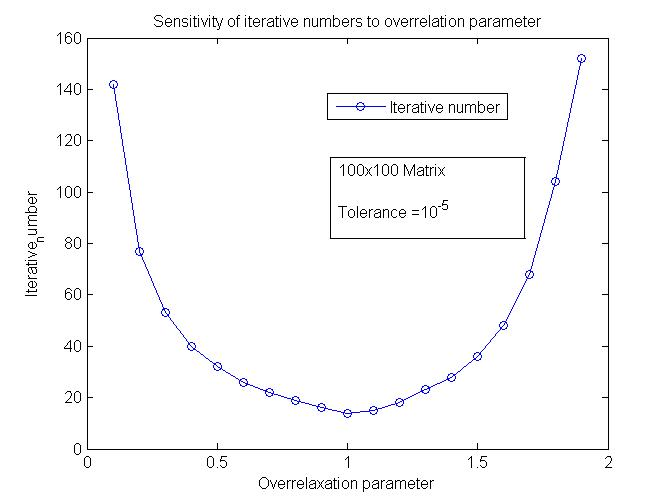
\includegraphics[height=3.5in,width=5in]{iterative_num_5.jpg}$\\
$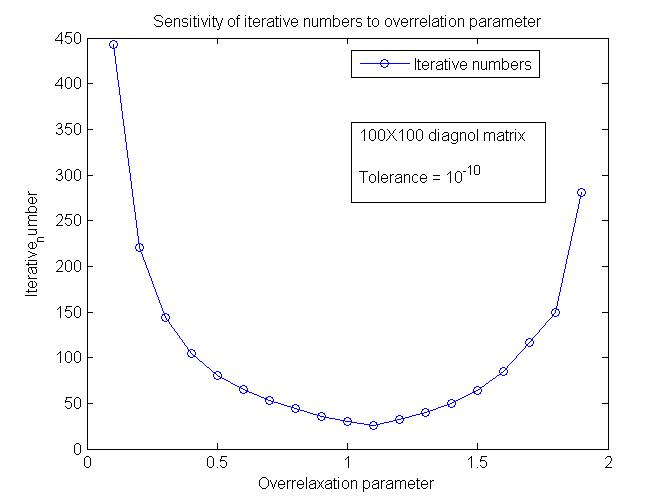
\includegraphics[height=3.5in,width=5in]{iterative_num_10.jpg}$\\

The above charts showed that the iteration number was first  decreasing with the increasing of the overrelation parameter, when the overrelaxation parameter was around 1.1, the iterative number started to increase.\\ The situation for tolerance $10^{-10}$ and tolerance $10^{-10}$ was similar.\\ We can also found that:\\
\begin{equation}
\rho=max\frac{\{(\frac{1}{\omega}-1)\left|d_i\right|+\left|u_i\right|\}}{\{\frac{\left|d_i\right|}{\omega}-l_i\}}=\frac{\{(\frac{1}{\omega}-1)\left|3\right|+\left|1\right|\}}{\{\frac{\left|3\right|}{\omega}-l_i\}}<1;
\end{equation}

So the convergence theorem holds and our PSOR solver works.\\

Our first problem is to redo the assignment 1 problem based on the POSR method and compute the CPU time. \\

So we set $E^*=\$10$, $r^*=0.05/yr$, $\sigma^*=0.20/yr$ T=0.5 as the example to build our model. \\
We watch the cpu time in the following two situation:\\
First under different overrelaxation parameter:\\
$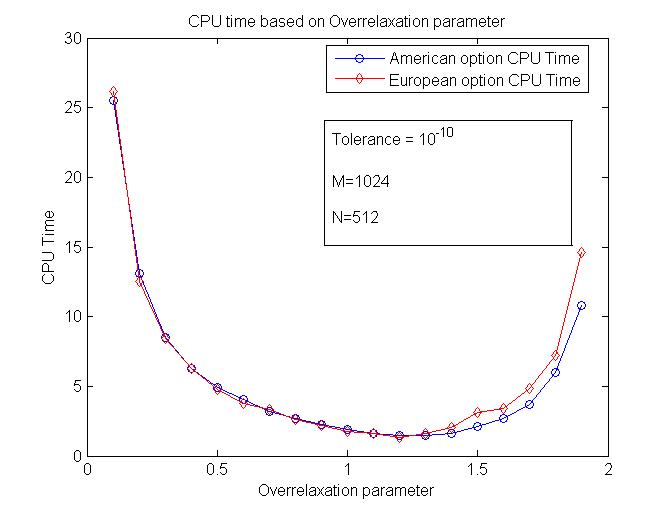
\includegraphics[height=3.5in,width=5in]{cpu_time_omega.jpg}$\\

The above figure showed that the cpu time for the European option was a little bit higher than American option on the small and big overrelaxation paramater, and a little bit lower around 1.The main reason may be that the American option need less iterative numbers to converge, when the $\omega$ was very high and low. Besides, both European and American Option reached the minimal CPU time around parameter 1.2.\\

$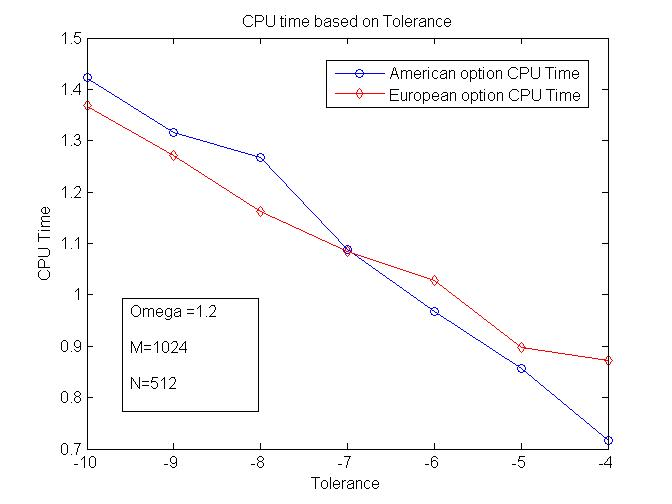
\includegraphics[height=3.5in,width=5in]{cpu_time_tol.jpg}$\\

The second situation is the tolerance, both American and European option CPU time decreased with the increasing of the tolerance.  The CPU time for American option is higher than the European when the tolerance was less than $10^{-7}$ and lower when the tolerance increased after that.\\

Next we try to see the influence of the mesh grid to CPU time. The tolerance was set as $10^{-10}$ and overrelaxation parameter was set as 1.2.\\
\begin{tabular}{|c|c|c|c|c|c|}
\hline
$N_x$&$N_t$&European&	Increasing ratio&	American&	Increasing ratio
\\
\hline
16&8&0.001486 &&0.001150 & \\
32&16&0.002443 &1.64 &0.002138 &1.86\\
64&32&0.005997 &2.45 &0.005571 &2.61\\
128&64&0.019255 &3.21 &0.015861 &2.85\\
256&128&0.063979 &3.32 &0.052949 &3.34\\
512&256&0.253021 &3.95 &0.202332 &3.82\\
1024&512&1.348758 &5.33 &1.467072 &7.25\\
\hline
\end{tabular}

With the increasing of the mesh grids, the CPU time is increasing, and the ratio of time change was also increasing, which meant that the computer consumed more as the grids increased.
\end{homeworkProblem}

\begin{homeworkProblem}
Now we try to see how many points we need to ensure that the numerical result would have 4 significant digits.\\
We set the $S_{max}$ equal to 8*S, $\omega=1.2$, and $Tol=10^{-10}$, In order to ensure 4 digit numbers, we need the relative error less than 0.00005.\\

First we set N equal to 160 and watch the relative error with the increasing of stock price steps.\\
$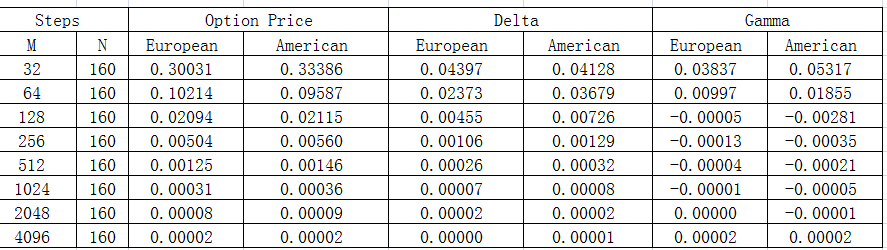
\includegraphics[height=2.2in,width=5.5in]{error160.png}$\\

When M increased to 4096, both European and American option ensure the 4 digit numbers.\\

Now we set the N equal to 320, the relative error was listed in the following:\\
$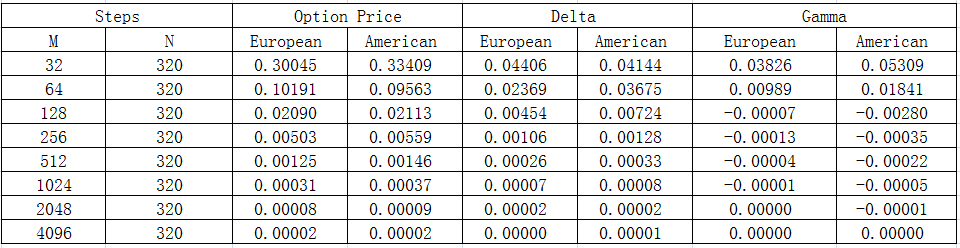
\includegraphics[height=2.2in,width=5.5in]{error320.png}$\\
The situation was similar, we still need 4096 ponts to ensure the 4 digit numbers.

Now we set M = 2048 and N = 1024 to see the results of the option price, delta and gamma under the PSOR methods\\
\textbf{[option price]}
\\
$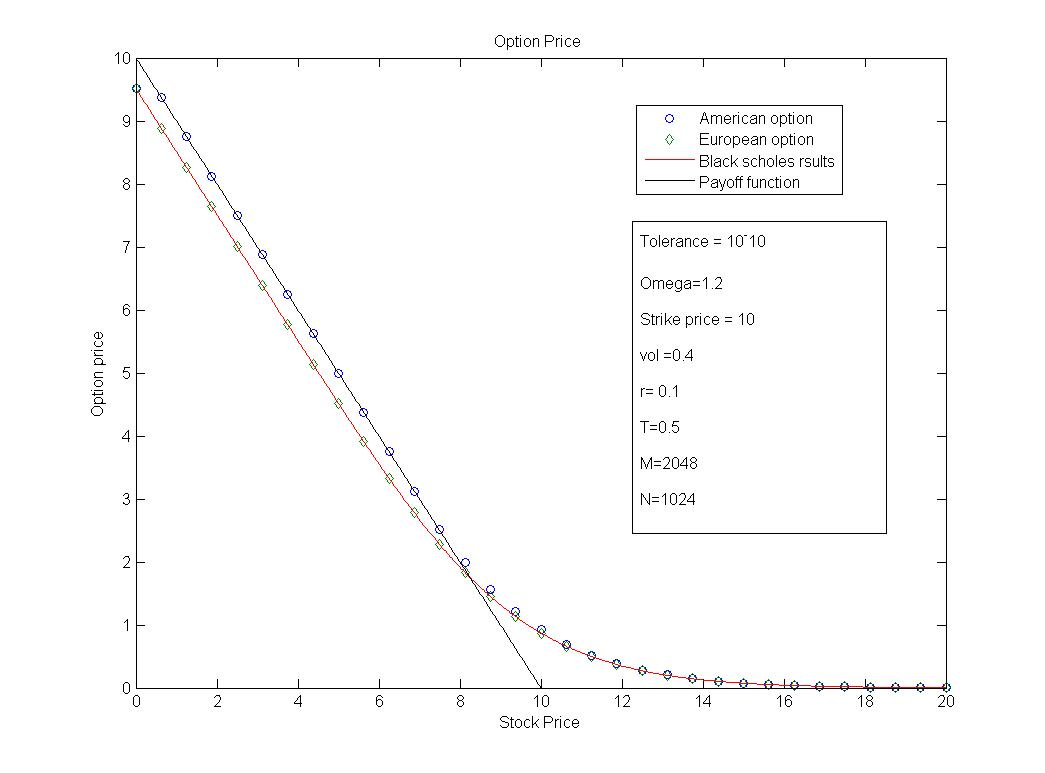
\includegraphics[height=4in,width=5.5in]{optionprice.jpg}$\\
We can see that American option price was higher than the European option, which made sense, since American put option had the inside early exercise right, so the value was more valuable.\\ From this chart,we can also find the phenomenon of the Optimal Exercise Boundary. 

We can see that the American put prices were same with the European put prices when the stock prices was bigger than Optimal Exercise Boundary $S_f$. When stock prices was less than $S_f$, American put option price was equal to the payoff function.\\
\textbf{[Delta]}
\\
$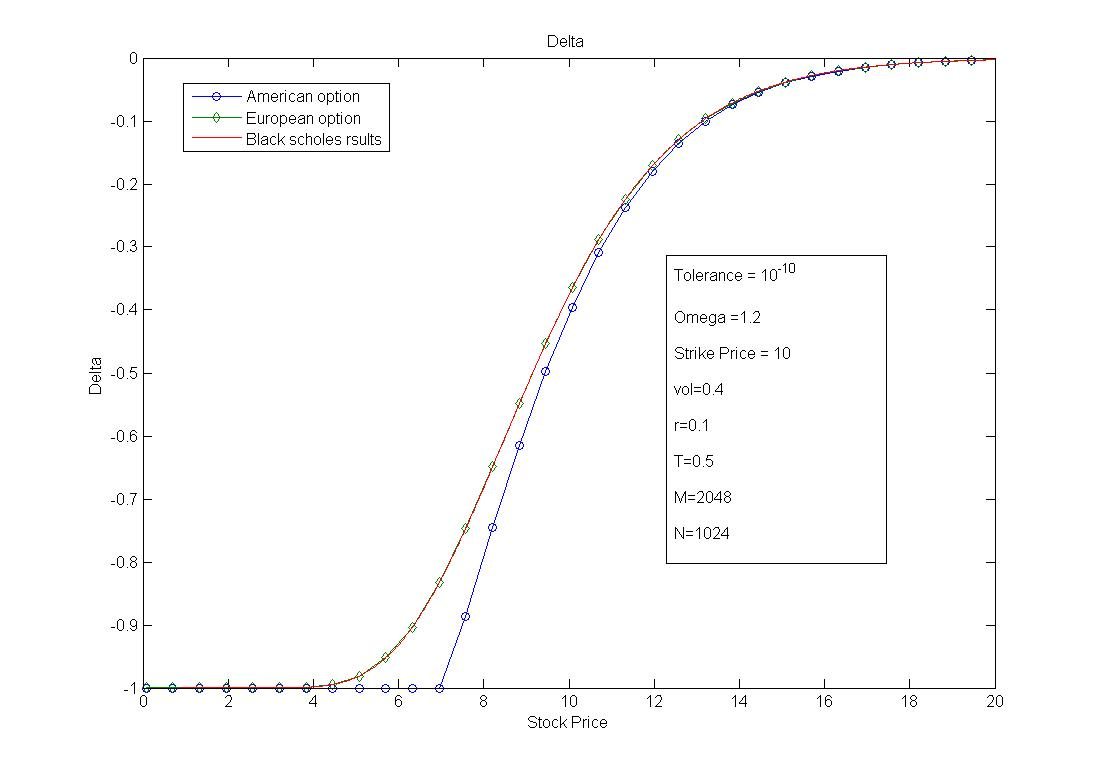
\includegraphics[height=4in,width=5.5in]{delta.jpg}$\\

Delta for the American put option was equal to -1, when stock prices was less than $S_f$\\
\textbf{[Gamma]}
\\
$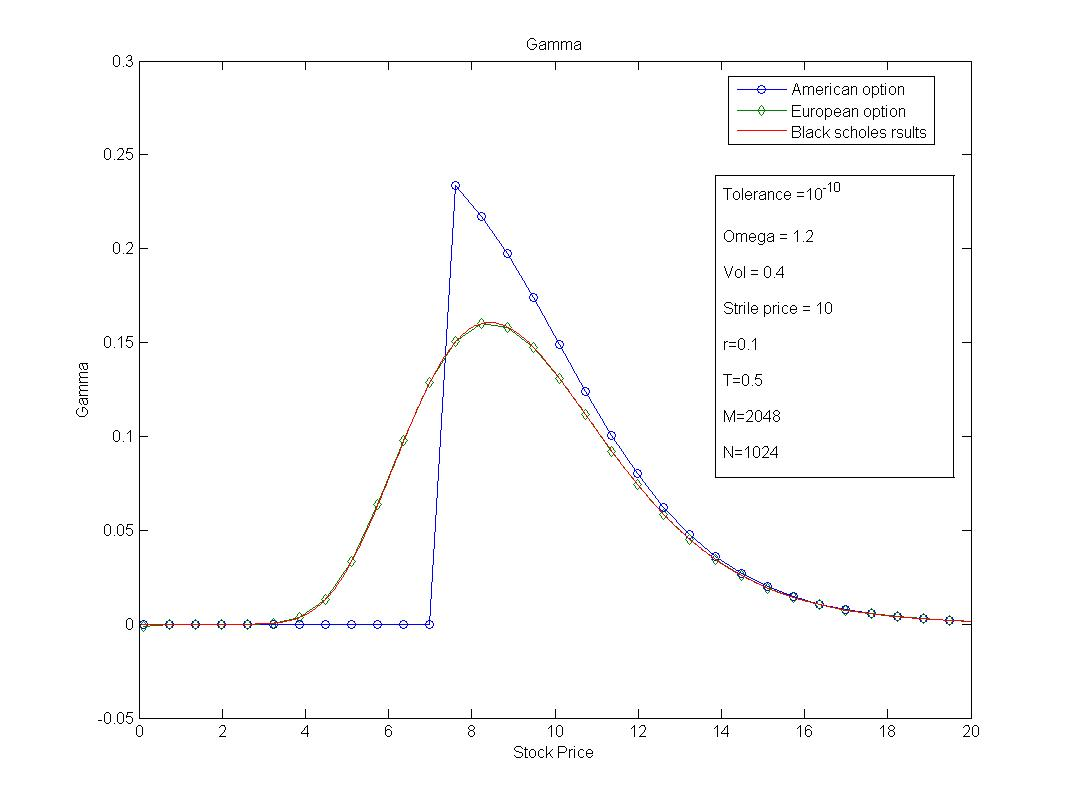
\includegraphics[height=4in,width=5.5in]{gamma.jpg}$\\

The gamma of American put option increased from 0 dramatically, when stock price was around $S_f$, it is because that the delta was increased from -1 to some higher value, when the stock price touched the $S_f$.\\

 
\end{homeworkProblem}

\begin{homeworkProblem}
We set tolerance equal to $10^{-10}$, $\omega$ equal to 1.2 ,M=2048 and N=1024, To see the optimal exercise boundary VS maturity time\\

$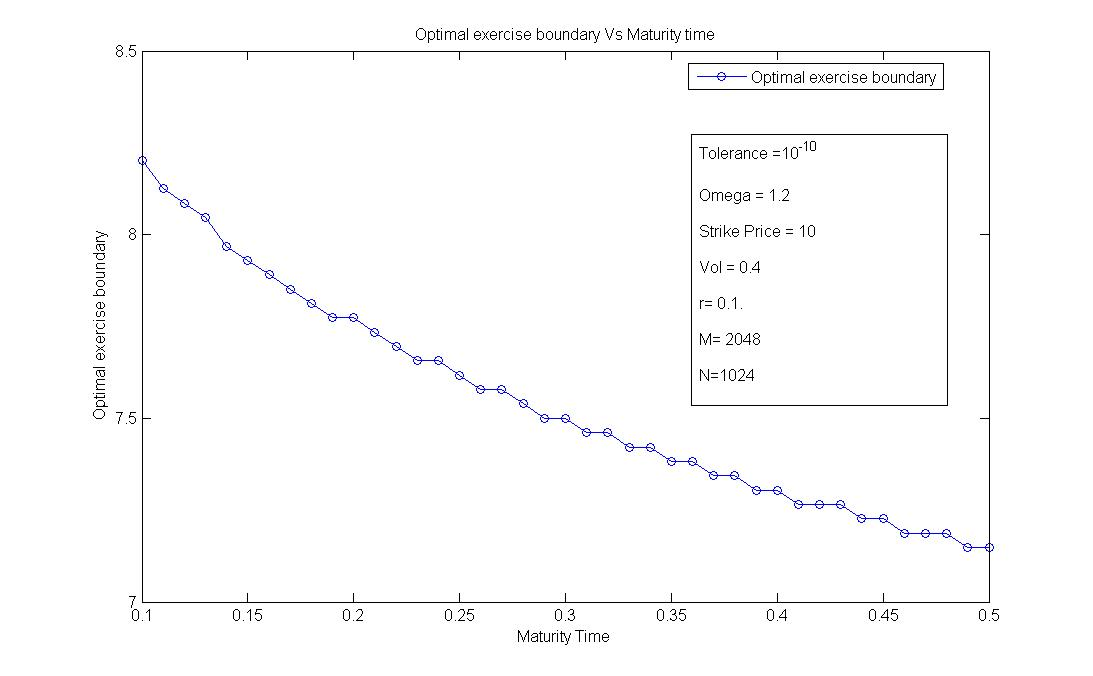
\includegraphics[height=4in,width=5.5in]{sf.jpg}$\\

From the above chart, we found when the maturity time increased, the optimal exercise boundary decreased, which meant that when time was close to the maturity time, the optimal exercise boundary would aproach to the strike price K which was 10 in this problem.\\

\end{homeworkProblem}
\end{document} 